\documentclass[12pt,a4paper]{article}

\usepackage{fontawesome5}
\providecommand{\faPencilAlt}{\faIcon{pencil-alt}}

\usepackage{styles/couleurs}
\usepackage{styles/mise_en_page}
\usepackage{styles/boites}
\usepackage{styles/maths}
\usepackage{styles/figures}

\usepackage{enumitem}
\usepackage{array}
\usepackage{tabularx}
\usepackage{amsmath}
\usepackage{amssymb}
\usepackage{tikz}
\usepackage{xparse}
\usepackage{pdflscape}
\usepackage{colortbl}

\usetikzlibrary{calc,arrows.meta,positioning}

\setlist[itemize]{leftmargin=1.4em,itemsep=0.15em,topsep=0.2em}
\setlist[enumerate]{leftmargin=*,itemsep=0.22em,topsep=0.25em}

\newcommand{\lignepointillee}{\noindent\dotfill\par\vspace{0.45em}}

\newcommand{\lignesreponse}[1]{%
\begin{tcolorbox}[
enhanced,colback=white,colframe=NeutreC!40,boxrule=0.5pt,arc=1.5mm,
left=3mm,right=3mm,top=2mm,bottom=1mm,before skip=2pt,after skip=2pt]
\foreach \i in {1,...,#1}{\lignepointillee}
\end{tcolorbox}}

\newcommand{\titreseq}[1]{%
\begin{center}
{\sffamily\large\bfseries\color{SavoirC}#1}
\end{center}}

\newcommand{\grillecent}{%
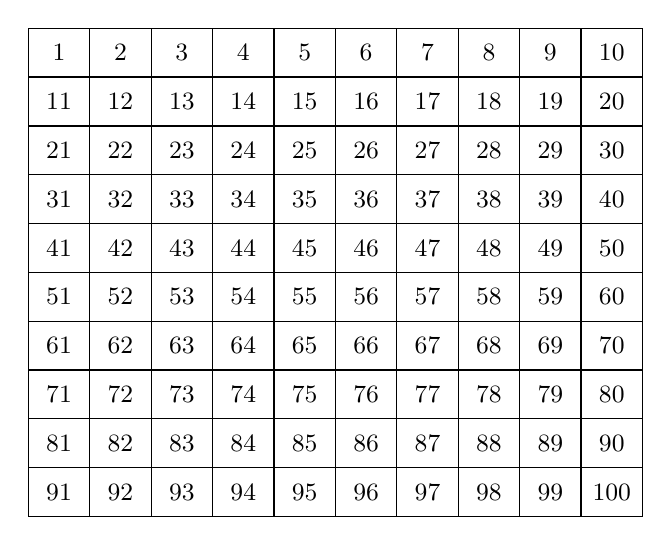
\begin{tikzpicture}[x=0.78cm,y=0.62cm]
  \foreach \n in {1,...,100}{
    \pgfmathtruncatemacro{\col}{mod(\n-1,10)}
    \pgfmathtruncatemacro{\lig}{9-floor((\n-1)/10)}
    \draw[line width=0.45pt] (\col,\lig) rectangle ++(1,1);
    \node[font=\small] at (\col+0.5,\lig+0.5) {\n};
  }
\end{tikzpicture}}

\begin{document}

\titreseq{Activité 2 -- Le jeu de Juniper Green}

\section*{Règles}

\begin{enumerate}
  \item Le premier joueur coche un nombre.
  \item À son tour, l'autre joueur coche un nombre encore libre
        qui est un \textbf{multiple ou un diviseur} du nombre précédent.
  \item Les joueurs poursuivent en alternance.
  \item Le joueur qui ne peut plus jouer perd la partie.
\end{enumerate}

\begin{center}
\grillecent
\end{center}
\section*{Analyser les coups}

\begin{enumerate}
  \item Après le nombre \(42\), quels nombres pourrait-on jouer ?
        Donne au moins quatre possibilités.
  \item Après le nombre \(37\), quels nombres pourrait-on jouer au début d'une partie ?
  \item Que se passe-t-il si le nombre \(1\) a déjà été utilisé
        et qu'un joueur choisit un nombre premier supérieur à \(50\) ?
  \item Pourquoi les nombres premiers ont-ils une place particulière dans ce jeu ?
\end{enumerate}

\lignesreponse{11}

\end{document}
